\documentclass{article}
\usepackage{v-test-paper}
\def\TITLE{Center of Mass and Collisions}


\title{\textsc{\TITLE}}
% \date{February 27, 2024}
\date{Day-8}
\usepackage[none]{hyphenat}
\usetikzlibrary{mindmap}
\usetikzlibrary {patterns,patterns.meta} 

\newcommand{\itemstared}{\refstepcounter{enumi}\item[$^\star$\theenumi.]}
\usetikzlibrary{matrix,  positioning, patterns, backgrounds}
\renewcommand{\ans}{\quad}
\renewcommand{\ansint}[1]{\underline{\hspace{2cm}}}


\tikzstyle{root} = [rectangle, rounded corners, 
minimum width=3cm, 
minimum height=0.7cm,
text centered, 
draw, 
font=\scshape,
]
\tikzstyle{child} = [rectangle, rounded corners, 
inner sep=2mm,
text centered, 
draw, 
font=\itshape,
text width=3.25cm,
]

\tikzstyle{child-branch} = [
    rectangle, 
    rounded corners, 
    inner sep=2mm,
    text centered, 
    draw, 
    font=\itshape,
    text width=2.75cm,
]
\tikzstyle{child-stared} = [
    rectangle, 
    rounded corners, 
    inner sep=2mm,
    text centered, 
    draw, 
    font=\itshape,
    text width=2.75cm,
    label={[anchor=north west]north west:*}
]

\tikzstyle{ball}=[
    circle, 
    minimum size=0.5cm, 
    draw, 
    shade,
]



\tikzstyle{arrow} = [thick,->,>=latex]


\begin{document}
\sloppy
\maketitle
\begin{center}
\begin{tikzpicture}
    
\def\root{\TITLE}
\def\RowOneColOne{Center Of Mass}
\def\RowOneColTwo{Collisions}
%\def\RowOneColThree{Understanding the concept of pseudo force}
\def\RowTwoColOneLeft{Definition and Calculation Position of Center of Mass}
\def\RowTwoColOneRight{Velocity of Center of Mass}
\def\RowTwoColTwoLeft{Elastic Collision}
\def\RowTwoColTwoRight{Inelastic Collision}
\def\RowThreeColOneLeft{Acceleration of Center of Mass}

\def\RowThreeColTwoLeft{Head on Collision, Oblique Collision}
\def\RowFourColOne{If $\vec{a}_{\textit{COM}}=0$, Conservation of Linear Momentum}
\def\RowFourColTwoRight{Linear Impluse}
\def\RowFourColTwoLeft{Variable Mass System(Rocket Propulsion)}

\matrix [column sep=-20mm,row sep=10mm]
{
&\node (root) [root] {\root};\\
\node (row_one_col_one)[child] {\RowOneColOne}; & &
\node (row_one_col_two)[child] {\RowOneColTwo}; \\
\node[child-branch](row_two_col_one_left)at ($(row_one_col_one.south)+(-2, 0)$){\RowTwoColOneLeft};
\node[child-branch] (row_two_col_one_right) at ($(row_one_col_one.south)+(2, 0)$){\RowTwoColOneRight};& &
\node[child-branch](row_two_col_two_left)at ($(row_one_col_two.south)+(-2, 0)$){\RowTwoColTwoLeft}; 
\node[child-branch](row_two_col_two_right) at ($(row_one_col_two.south)+(2, 0)$){\RowTwoColTwoRight};\\
\node[child-branch] (row_three_col_one_left) at ($(row_two_col_one_right.south)+(0, 1)$){\RowThreeColOneLeft};
 & &
\node[child-branch] (row_three_col_two_left)at ($(row_two_col_two_left.south)+(2, 1)$){\RowThreeColTwoLeft};\\
\node[child-branch] (row_four_col_one) at ($(row_three_col_one_left.south)+(0, 1)$){\RowFourColOne};&&
\node[child-stared] (row_four_col_two) at ($(row_three_col_one_left.south)+(0, 1)$){\RowFourColTwoLeft};
\node[child-stared] (row_four_col_two_right) at ($(row_three_col_one_left.south)+(-3.5, 1)$){\RowFourColTwoRight};\\
};

\draw[arrow](root.west)-|(row_one_col_one.north);
\draw[arrow](root.east)-|(row_one_col_two.north);
\draw[arrow](row_one_col_one)--(row_two_col_one_left);
\draw[arrow](row_one_col_one)--(row_two_col_one_right);
\draw[arrow](row_one_col_two)--(row_two_col_two_left);
\draw[arrow](row_one_col_two)--(row_two_col_two_right);
\draw[arrow](row_two_col_one_right)--(row_three_col_one_left);
\draw[arrow](row_two_col_two_left)--(row_three_col_two_left);
\draw[arrow](row_two_col_two_right)--(row_three_col_two_left);
%\draw[arrow](row_three_col_two_left)--(row_four_col_two);
\draw[arrow](row_three_col_one_left)--(row_four_col_one);
\end{tikzpicture}
\end{center}

\begin{center}
    \textsc{Problems}
\end{center}
\begin{enumerate}

    \item A rocket of mass $m_0$ has attained a speed equal to its exhaust speed and at that time the mass of
    the rocket is $m$. Then the ratio $\dfrac{m_0}{m}$ is (neglect gravity)
    \begin{tasks}(2)
        \task $2.718$\ans
        \task $7.8$
        \task $3.14$
        \task $4$
    \end{tasks}

    \item A ball is moving with a velocity of $2\mps$ towards a heavy wall moving towards the ball with a velocity of $1\mps$ as shown in the figure. Assuming collision to be elastic, find the velocity of the ball immediately after the collision.
    \begin{center}
        
\begin{tikzpicture}
            \tzlines+[pattern=bricks](1, 0)(-1, 0)(0, 2.5)(1, 0);
            \node[ball] (ball) at (-4, 1.25){};
            \tzline+[->](ball.east)(1, 0){$2\mps$}[a]
            \tzline+[->](0, 1.25)(-1, 0){$1\mps$}[a] 
        \end{tikzpicture}
    \end{center}
    \begin{tasks}(2)
        \task $1.5\mps$
        \task $2.5\mps$
        \task $3\mps$
        \task $4\mps$\ans
    \end{tasks}

    \item A particle of mass $m$ is moving with a velocity $u$ makes an elastic one-dimensional collision  with a stationary particle of mass $m$. Their force of interaction increases from zero to $F_0$ linearly in time $0.5t_0$, and decreases linearly to zero in further time $0.5t_0$ as shown in figure. The magnitude of $F_0$ is
    \begin{center}
        \begin{tikzpicture}
            \tzaxes(0, 0)(5, 3){$t$}{$F$}
            \tzlines(0, 0)(2, 2)(4, 0);
            \tzticks{2/$0.5t_0$}{2/$F_0$}
            \tzlines+[dashed](2, 0)(0, 2)(-2, 0);
        \end{tikzpicture}
    \end{center}
    \begin{tasks}(2)
        \task $\dfrac{mu}{t_0}$
        \task $\dfrac{2mu}{t_0}$\ans
        \task $\dfrac{mu}{2t_0}$
        \task None of these
    \end{tasks}

    \item The figure shows a metallic plate of uniform thickness and density. The value of $l$ in terms of $L$ so that the center of mass of the system lies at the interface of the triangular and rectangular portion is
    \begin{center}
        \begin{tikzpicture}
            \tzrectangle[pattern=north east lines](0, 0)(4, 2)
            \tzlines+[pattern=north west lines](0, 2)(2, 1.5)(2, -1.5);
            \tzline+[|<->|]<0.5, 0>(4, 0)(0, 2){$l$}[mr]
            \tzline+[|<->|]<0.5, 0>(4, 2)(0, 1.5){$L$}[mr]
            \tzline+[|<->|]<0, -0.5>(0, 0)(4, 0){$b$}[mb]
        \end{tikzpicture}
    \end{center}
    \begin{tasks}(2)
        \task $l=\dfrac{L}{3}$
        \task $l=\dfrac{L}{2}$
        \task $l=\dfrac{L}{\sqrt{3}}$\ans
        \task $l=\sqrt{\dfrac{2}{3}}L$
    \end{tasks}


    \item The coefficient of friction between the horizontal surface and each of the block shown in the figure is $0.2$. The collision between the blocks is perfectly elastic. Find the separation between them when they come to rest. (Ignore the dimensions of the blocks and take $g=10\mpss$)
    \begin{center}
        \begin{tikzpicture}
            \pic (surface) {frame=8cm};
            \tzcoor(surface-center)(O)
            \node[block, anchor=south] (block1) at ($(O)+(-2.5, 0)$) {$2 \kg$};
            \node[block, anchor=south] (block2) at ($(O)+(2.5, 0)$) {$4 \kg$};
            \tzline+[->](block1.east)(1, 0){$1 \mps$}[r]
            \tzline[|<->|]<0, -0.5>(block1.south)(block2.south){$16\cm$}[mb]
        \end{tikzpicture}
    \end{center}
    \begin{tasks}(2)
        \task $8\cm$
        \task $12\cm$
        \task $16\cm$
        \task $5\cm$\ans
    \end{tasks}


    \item The density of a thin rod of length $L$ varies with the distance $x$ from one end as $\rho(x)=\uprho_0\dfrac{x^2}{L^2}$. The center of mass of the rod is at a distance $d$ from the end where the density is $\uprho_0$. The value of $d$ is
    \begin{center}
        \begin{tikzpicture}
            \tzline[line width=2.5mm, cap=round](0, 0)(6, 0)
            \tzline[|->]<0, -0.5>(6, 0)(4, 0){$d$}[midway, b]
            \tzline[|<->|]<0, 0.5>(0, 0)(6, 0){$L$}[midway, a]
            \tzdot*[white](4, 0)
        \end{tikzpicture}
        \end{center}
    \begin{tasks}(2)
        \task $\dfrac{L}{4}$\ans
        \task $\dfrac{L}{2}$
        \task $\dfrac{2L}{3}$
        \task $\dfrac{3L}{4}$
    \end{tasks}

    \item  Two blocks $A$ and $B$ of equal masses are released on two sides of a fixed wedge as shown in the figure. Find the acceleration  of the center of mass of the system. (Take $g=10\mpss$, Ignore friction) 
    \begin{center}
        \begin{tikzpicture}
            \pic (surface) {frame=9cm};
            \tzcoor(surface-center)(O)
            \tzcoor(-2.5, 0)(A)
            \tzcoor(-2.5 + 4*cosec{45}, 0)(B)
            \tzlines+(A)(45:4)(-45:4);
            \tzanglemark(O)(A)($(A)+(45:4)$){$45^\circ$}(16pt)
            \tzanglemark($(B)+(135:4)$)(B)(O){$45^\circ$}(15pt)
            \node[block, anchor=south, rotate=45] (block1) at ($(A)+(45:2)$){$A$};
            \node[block, anchor=south, rotate=-45] (block2) at ($(B)+(135:2)$){$B$};
        \end{tikzpicture}
    \end{center}
    \begin{tasks}(2)
        \task $10\mpss$
        \task $15\mpss$
        \task $5\mpss$\ans
        \task $20\mpss$
    \end{tasks}

    \item A ball of mass $m=1\kg$ strikes a smooth horizontal floor as shown in the figure. The impulse of the force exerted on the floor is
    \begin{center}
        \begin{tikzpicture}
            \pic (surface) {frame=8cm};
            \tzcoor(surface-center)(O)
            \tzcoor($(O)+(140:3)$)(A)
            \tzcoor($(O)+(30:3)$)(B)
            \tzdot*(A)(12pt)
            \tzline+[->](A)(-40:1){$5\mps$}[r]
            \tzline+[->, dashed](O)(30:3)
            \tzline+[dashed]($(O)+(140:3)$)(-40:3)
            \tzanglemark(A)(O)($(O)+(-1, 0)$){$53^\circ$}(15pt)
            \tzanglemark($(O)+(1, 0)$)(O)(B){$37^\circ$}(15pt)
        \end{tikzpicture}
    \end{center}
    \begin{tasks}(2)
        \task $6.25\N\s$\ans
        \task $1.76\N\s$
        \task $7.8\N\s$
        \task $2.2\N\s$
    \end{tasks}

    \item There is a system of six similar particles of mass $m$ each, placed on the vertices of a uniform hexagon of side $a$. The center of mass of the system is at its geometrical center. Now, one of the particles is removed from the system. The new position of the center of mass is at a distance $d$ from the center of the hexagon. The value of $d$ is
    \begin{center}
        \begin{tikzpicture}
            \foreach \i in {0, 60, ..., 300}
            {
                \tzcoor*({cos(\i)*2}, {sin(\i)*2})(P)(5pt)
                \tzcoor*({cos(\i+60)*2}, {sin(\i+60)*2})(Q)(5pt)
                \tzline[dashed](0, 0)(P)
                \tzline[dashed](P)(Q)
            }
        \end{tikzpicture}
    \end{center}

    \begin{tasks}(2)
        \task $\dfrac{a}{\sqrt{3}}$
        \task $\dfrac{a}{5}$\ans
        \task $\dfrac{a}{6}$
        \task $\dfrac{a}{3}$
    \end{tasks}

    \item A circular coil of radius $R$ made up of two different metals of different densities upper half with $\lambda_1$ and lower half $\lambda_2$. The center of mass of the coil is at a distance $d$ from the center of the coil. The value of $d$ is 
    \begin{tasks}(2)
        \task $\dfrac{2R}{\pi}\left(\dfrac{\lambda_1+\lambda_2}{\lambda_1-\lambda_2}\right)$
        \task $\dfrac{2R}{\pi}\left(\dfrac{\lambda_1}{\lambda_2}\right)$
        \task $\dfrac{2R}{\pi}\left(\dfrac{\lambda_2}{\lambda_1}\right)$
        \task $\dfrac{2R}{\pi}\left(\dfrac{\lambda_1-\lambda_2}{\lambda_1+\lambda_2}\right)$\ans
    \end{tasks}






    \begin{center}
        \textsc{Matrix Match Type}
    \end{center}

    \item Two blocks of masses $3 \kg$ and $6 \kg$ are connected by an ideal spring and are placed on a frictionless horizontal surface. The $3 \kg$ block is imparted a speed of $2 \mps$ towards left. (consider left as positive direction)
    \begin{center}
        \begin{tikzpicture}
            \pic (surface) {frame=8cm};
            \tzcoor(surface-center)(O)
            \node[block, anchor=south] (block1) at ($(O)+(-2, 0)$) {$3 \kg$};
            \node[block, anchor=south] (block2) at ($(O)+(2, 0)$) {$6 \kg$};
            \tzsnake[thick]{5pt}[coil, amplitude=5pt, pre length=7pt, post length=7pt](block1.east)(block2.west)
            \tzline+[->](block1.west)(-1, 0){$2 \mps$}[l]
        \end{tikzpicture}
    \end{center}
    \begin{center}
        \renewcommand{\arraystretch}{2}
        \begin{table}[h]
            \centering
            \begin{tabular}{p{0.25cm}p{7cm}|p{0.25cm}p{6cm}}
            \hline
            & Column I & &Column II \\
            \hline
            (a)& When the velocity of $3\kg$ block is $\dfrac{2}{3}\mps$ & (p) &Velocity of center of mass is $\dfrac{2}{3}\mps$\\
            (b)& When the velocity of $6\kg$ block is $\dfrac{2}{3}\mps$ & (q) &Deformation of the spring is zero\\
            (c)& When the speed of $3\kg$ block is minimum  & (r) &Deformation of the spring is maximum\\
            (d)& When the speed of $6\kg$ block is maximum & (s) &Both the blocks are at rest with respect to each other\\
            \hline
            \end{tabular}
        \end{table}
    \end{center}
    \begin{tasks}
        \task $a \rightarrow (p,r,s), ~b \rightarrow (p,r,s), ~c \rightarrow (p), ~ d\rightarrow (p,q)$\ans
        \task $a \rightarrow (p,r,s), ~b \rightarrow (p,r,s), ~c \rightarrow (p,q), ~ d\rightarrow (p)$
        \task $a \rightarrow (p,r,s), ~b \rightarrow (p,s), ~c \rightarrow (p), ~ d\rightarrow (p)$
        \task $a \rightarrow (p), ~b \rightarrow (p,r,s), ~c \rightarrow (p), ~ d\rightarrow (p,q)$
    \end{tasks}
    
    \begin{center}
        \textsc{Comprehension Based Questions}
    \end{center}
    {\textbf{Passage I[12 to 14]}}\\
    There is a system of trolley and a conical pourer(through which sand can be poured into the trolley) as shown in the figure. A constant force $F$ is applied on a trolley of initial mass $m_0$ kept over a smooth surface. Sand is poured gently over the trolley at a constant rate of $\upmu \kg/\s$. Based on above information answer the following questions.
    \begin{center}
        \begin{tikzpicture}
            \def\R{0.25}
            \def\L{4}
            \def\H{1.5}
            \pic (surface) {frame=8cm};
            \tzcoor(surface-center)(O)
            \tzcoor*($(O)+(-0.3*\L, \R)$)(C1)
            \tzcoor*($(O)+(0.3*\L, \R)$)(C2)
            \tzcoor($(O)+(-0.5*\L, 2*\R)$)(LC)
            \tzrectangle+(LC)(\L, \H)
            \tzcircle(C1)(\R)
            \tzcircle(C2)(\R)
            \tzline+[->]($(O)+(0.5*\L, 0.5*\H + 2*\R)$)(1, 0){$F$}[r]
            \tzlines+($(O)+(-1.5*\R, 2*\R+\H)$)(\R, \R)(0, 2*\R)(-2*\R, 2*\R);
            \tzlines+($(O)+(1.5*\R, 2*\R+\H)$)(-\R, \R)(0, 2*\R)(2*\R, 2*\R);
            \tzlines+[pattern={Dots[radius=1.5pt, angle=45]},pattern color=black, draw=none]($(O)+(-1.5*\R, 2*\R+\H)$)(\R, \R)(0, 2*\R)(-2*\R, 2*\R)(5*\R, 0)(-2*\R, -2*\R)(0, -2*\R)(\R, -\R);
        \end{tikzpicture}
    \end{center}
    \item After time $t$, the velocity of trolley is
    \begin{tasks}(2)
        \task $v=\dfrac{Ft}{m_0+\upmu t}$\ans
        \task $v=\dfrac{Ft}{m_0-\upmu t}$
        \task $v=\dfrac{2Ft}{m_0+\upmu t}$
        \task $v=\dfrac{2Ft}{m_0-\upmu t}$
    \end{tasks}

    \item Net force acting on the trolley as a function of time is
    \begin{tasks}(2)
        \task $F_{\textit{net}}=\dfrac{Fm_0}{m_0-\upmu t}$
        \task $F_{\textit{net}}=\dfrac{Fm_0}{m_0+\upmu t}$\ans
        \task $F_{\textit{net}}=\dfrac{2Fm_0}{m_0+\upmu t}$
        \task $F_{\textit{net}}=\dfrac{2Fm_0}{m_0-\upmu t}$
    \end{tasks}

    \item Mass of the trolley at time $t$ is
    \begin{tasks}(2)
        \task $m_0-\upmu t$
        \task $2m_0+\upmu t$
        \task $2m_0-\upmu t$
        \task $m_0+\upmu t$\ans
    \end{tasks}

    {\textbf{Passage II[15 to 17]}}\\
    A ball of mass $M$ is suspended from a massless string of length $l$ as shown in figure. A bullet of mass $m$ moving with velocity $v_0$ collides with the ball and sticks with the ball. Now, velocity of the combined mass $(M + m)$ just after collision at the bottom most point can be obtained from law of conservation of linear momentum. Based on above information answer the following questions.
    \begin{center}
        \begin{tikzpicture}
            \def\L{3}
            \def\R{0.25}
            \pic[rotate=-180] (surface) {frame=2cm};
            \tzcoor(surface-center)(O)
            \tzline+(O)(0, -3){$l$}[mr]
            \tzcircle[fill=black]($(O)+(0, -\L-\R)$)(\R)
            \tzcoor*($(O)+(-0.8*\L, -\L-\R)$)(m){$m$}[a](5pt)
            \tzline+[->](m)(1, 0){$v_0$}[r]
            \tznode($(O)+(\R, -\L-\R)$){$M$}[r]
        \end{tikzpicture}
    \end{center}
    \item Velocity of the combined mass $(M + m)$ just after collision at the bottom most point is
    \begin{tasks}(2)
        \task $\dfrac{Mv_0}{M+m}$
        \task $\dfrac{2mv_0}{M+m}$
        \task $\dfrac{2Mv_0}{M+m}$
        \task $\dfrac{mv_0}{M+m}$\ans
    \end{tasks}

    \item Loss of mechanical energy during the collision is
    \begin{tasks}(2)
        \task $\dfrac{Mmv_0^2}{2(M+m)}$\ans
        \task $\dfrac{Mmv_0^2}{M+m}$
        \task $\dfrac{Mmv_0^2}{2M}$
        \task $\dfrac{Mmv_0^2}{2m}$
    \end{tasks}

    \item Minimum value of $v_0$ for which the combined mass will complete the vertical circular motion is
    \begin{tasks}(2)
        \task $\dfrac{m}{M-m}\sqrt{5gl}$
        \task $\dfrac{m}{M+m}\sqrt{5gl}$
        \task $\dfrac{M+m}{m}\sqrt{5gl}$\ans
        \task $\dfrac{M-m}{m}\sqrt{5gl}$
    \end{tasks}

    {\textbf{Passage III[18 to 20]}}\\
    A projectile is launched with an initial speed of \(v_0\), achieving a range of \(R_0\), a maximum height of \(H_0\), and a time of flight of \(T_0\). Upon collision with the surface, instead of coming to rest, the projectile bounces back due to the inelastic nature of the collision. This bouncing back is a recursive process, where the projectile continues to follow a projectile motion after each bounce. The coefficient of restitution, denoted by \(e\), between the surface and the ball determines the velocity with which the projectile bounces back. This coefficient, a ratio of the final to initial relative velocity between two objects after they collide, influences the subsequent range, maximum height, and time of flight for each successive bounce. Based on above information answer the following questions.
    \begin{center}
        \begin{tikzpicture}
            \tzaxes(0, 0)(9, 3){$x$}{$y$}
            \tzparabola(0, 0)(1.5, 1.5)(3, 0)
            \tzparabola(3, 0)(4, 1)(5, 0)
            \tzparabola(5, 0)(5.8, 0.5)(6.6, 0)
            \tzparabola(6.6, 0)(7.2, 0.3)(7.8, 0)
            \tzline+[->](0, 0)(1, 0){$u_x$}[b]
            \tzline+[->](0, 0)(0, 1){$u_y$}[l]
        \end{tikzpicture}
    \end{center}
    \item The range of the projectile after the $n^{\textit{th}}$ bounce is
    \begin{tasks}(2)
        \task $R_0$
        \task $R_0(1+e)^n$
        \task $R_0(1-e)^n$
        \task $R_0e^n$\ans
    \end{tasks}

    \item The maximum height of the projectile after the $n^{\textit{th}}$ bounce is
    \begin{tasks}(2)
        \task $H_0e^n$
        \task $H_0(1+e)^{2n}$
        \task $H_0(1-e)^{2n}$
        \task None of these\ans
    \end{tasks}

    \item The time of flight of the projectile after the $n^{\textit{th}}$ bounce is
    \begin{tasks}(2)
        \task $T_0e^{2n}$
        \task $T_0e^n$\ans
        \task $T_0(1-e)^n$
        \task $T_0(1+e)^n$
    \end{tasks}


    
    

    

\end{enumerate}

% \begin{center}
%     \textsc{Integer Type}
% \end{center}

% \begin{enumerate}\addtocounter{enumi}{17}
%     \item In the figure shown, all surfaces are smooth and force constant of spring is $10 \N/\m$. Block of mass $2 \kg$ is not attached with the spring. The spring is compressed by $2\m$ and then released. Find the maximum distance $d$ travelled by the block over the inclined plane. Take ($g = 10 \mpss$) .\ansint{2}
%     \begin{center}
%     \begin{tikzpicture}
%         \fill[pattern=north east lines](-0.25, -0.25)--(-0.25, 1.5)--(0, 1.5)--(0, 0)--(6, 0)--(8.6, 1.5)--(8.6, -0.25)--cycle;
%         \draw[thick](0, 1.5)--(0, 0)--(6, 0)--(8.6, 1.5);
%         \node[block] (block) at (3, 0.4) {$m$};
%         \tzline+[->](block.east)(1, 0){$v$}[r]
%         \tzsnake{5pt}[coil, amplitude=5pt, pre length=5pt, post length=0pt](0,0.4){$k$}[a=2mm](block.west)
%         \tzanglemark[thick, ->](8.6, 0)(6, 0)(8.6, 1.5){$30^\circ$}[fill=white, inner sep=1pt](25pt)
%         \tzline+[dashed](6, 0)(2, 0)
%     \end{tikzpicture}
%     \end{center}

% \end{enumerate}


\pagebreak
% \vspace*{\fill}

\begin{center}
\texttt{Answer Key}
\begin{multicols}{5}
\begin{enumerate}
\item (b)
\item (b)
\item (a)
\item (b)
\item (d)
\item (b)
\item (c)
\item (a), (b)
\item (c)
\item (a), (b), (c), (d)
\end{enumerate}
\end{multicols}
\end{center}


% % \begin{figure}[h]
% %     \rotatebox{180}{
% %     \begin{minipage}{\textwidth}
% %         \begin{center}
\texttt{Answer Key}
\begin{multicols}{5}
\begin{enumerate}
\item (b)
\item (b)
\item (a)
\item (b)
\item (d)
\item (b)
\item (c)
\item (a), (b)
\item (c)
\item (a), (b), (c), (d)
\end{enumerate}
\end{multicols}
\end{center}

% %     \end{minipage}
% %     }
% %     \end{figure}



\end{document}